%% このファイルは sample.md から pandoc で生成したものです（make latex/sample.tex）。
%% 直接編集せず、sample.md を編集してください。
\documentclass[paper]{bunkajoho}

\addbibresource{sample.bib}

%% pandoc の出力に必要な定義
\providecommand{\tightlist}{%
  \setlength{\itemsep}{0pt}\setlength{\parskip}{0pt}}

\title{紀要「文化情報学」テンプレートの設計}
\subtitle{執筆要項に基づくクラスファイルと文献スタイル}
\author{同志社 太郎・文化 花子}

\begin{abstract}
本稿は、同志社大学文化情報学会紀要『文化情報学』の執筆要項（2022 年 12 月 7 日改訂）に基づいて作成したテンプレートの使い方を示すものである。本文そのものが使用例となっており、タイトルページの構成、節番号、図表、数式、脚注、参照文献の書き方を順に説明する。要旨は和文・英文いずれで書いてもよい。
\end{abstract}

\begin{document}
\maketitle

\section{はじめに}

執筆要項では、掲載論文は LaTeX または Microsoft Word で作成し、編集委員会が用意したスタイルファイルを用いることとされている。本テンプレートはその叩き台であり、1 つの Markdown ファイル（sample.md）から
LaTeX 版（sample.tex）と Word 版（sample.docx）の両方を生成する。先頭のメタデータの \texttt{type} で種別（研究論文・研究ノート・資料紹介・書評）を切り替えると、第 1 ページ左上の種別ラベルが変わる。

第 1 ページには、要項 4. のとおり、タイトル・種別・著者名・アブストラクトが置かれる。ページ番号は事務局が付けるため、投稿原稿には付けない。

\section{本文の書き方}

\subsection{節と項}

本文は節から構成し、各節には 1、2.3、3.4.2 のように番号を付ける（要項 5.）。
Markdown では \texttt{\#}、\texttt{\#\#}、\texttt{\#\#\#} の見出しがそれぞれに対応し、番号は自動で付く。

\subsubsection{表記上の注意}

日本語で執筆する場合、句読点は「、」と「。」を用いる。専門用語は原則として日本語で表記し、必要なら初出時のみ欧文を丸括弧内に併記する。たとえば「アフォーダンス（affordance）」のように書く。略語は初出時に正式名を記し、続けて丸括弧内に略語を示す。たとえば「大規模言語モデル（Large Language Model; LLM）」とする。

\subsection{数式}

数式は別行に記し、末尾に通し番号を付ける。
\begin{equation}
  H(X) = -\sum_{i=1}^{n} p(x_i) \log_2 p(x_i)
\end{equation}
本文中に埋め込む場合には、\(a/b\)、\(\exp(x/y)\)、\(\delta x/\delta t\) のような記法を用いる。式番号は式 (2) のように参照する。
\begin{equation}
  I(X;Y) = H(X) - H(X \mid Y)
\end{equation}

\subsection{注}

注はなるべく用いない\footnote{止むを得ず使用する場合は、このように脚注で書く。刷り上がりではすべて脚注となる。}。

\section{図表}

図表には「図 1」「表 1」のように通し番号を付け、キャプションは原則として日本語で書く（要項 6.）。図 1 と表 1 に例を示す。査読用原稿では図表を本文中に埋め込んで提出し、採択後の最終原稿では図の相当部分を空白にして充分な解像度のデータを別途提出する（要項 4.）。他の文献から転載する場合は、著作権者の了解を得たうえで出典を明記する。

\begin{figure}[tb]
  \centering
  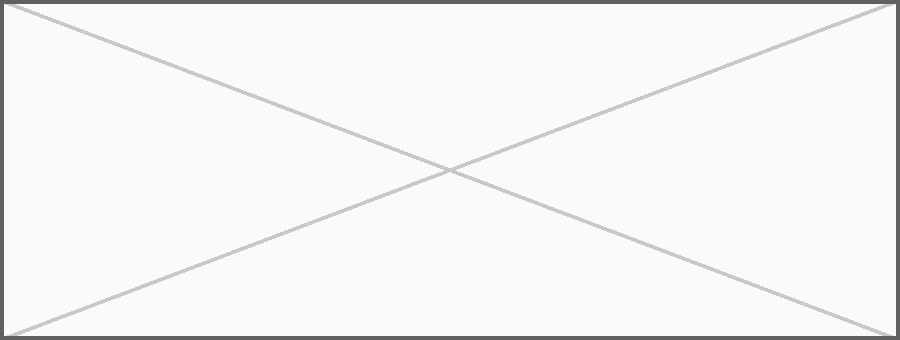
\includegraphics[width=0.90\linewidth]{figure1.png}
  \caption{図の例}
\end{figure}

\begin{table}[tb]
  \centering
  \caption{表の例}
  \begin{tabular}{lrr}
    \toprule
    項目 & 度数 & 割合（\%） \\
    \midrule
    研究論文 & 12 & 60.0 \\
    研究ノート & 5 & 25.0 \\
    書評 & 3 & 15.0 \\
    \bottomrule
  \end{tabular}
\end{table}

\section{参照文献}

本文中で文献を参照する際は、著者の姓の後に発表年を西暦で記す（要項 7.）。表 2 に要項の例と対応する Markdown の書き方を示す。

\begin{table*}[tb]
  \centering
  \caption{引用の書き方と出力}
  \footnotesize
  \begin{tabular}{ll}
    \toprule
    Markdown & 出力 \\
    \midrule
    \texttt{@gibson1979} & \textcite{gibson1979} \\
    \texttt{{[}@saeki1990{]}} & \autocite{saeki1990} \\
    \texttt{@haugeland1987\ {[}p.123{]}} & \textcite[123]{haugeland1987} \\
    \texttt{Simon\ {[}-@simon1973;\ -@simon1981{]}} & Simon \autocite*{simon1973,simon1981} \\
    \texttt{{[}@simon1973;\ @simon1981{]}} & \autocite{simon1973,simon1981} \\
    \texttt{@cohen1990a} & \textcite{cohen1990a} \\
    \texttt{{[}@cohen1990a;\ @cohen1990b{]}} & \autocite{cohen1990a,cohen1990b} \\
    \texttt{{[}@anzai1992;\ @joshi1981;\ @minsky1975;\ @minsky1986{]}} & \autocite{anzai1992,joshi1981,minsky1975,minsky1986} \\
    \bottomrule
  \end{tabular}
\end{table*}

文章の一部として読む場合は \textcite{gibson1979} によれば\ldots\ldots のように書き、そうでない場合は\ldots\ldots が提唱されている\autocite{saeki1990}のように書く。

文献リストは「文献」という見出しのもとに出力される。欧文と和文を区別せず、第 1 著者の姓のアルファベット順に並び、番号は付かない。和文文献には bib ファイルで \texttt{langid\ =\ \{japanese\}} を付け、正しい位置に並ぶよう \texttt{sortname} にローマ字読みを書き、キーもローマ字（姓＋年）にする。以下は要項に挙げられた例をすべて引用したものである：
\textcite{miller1956}、\textcite{cohen1985}、Minsky \autocite*{minsky1986,minsky1986b}、\textcite{saeki1990}、
\textcite{minsky1975}、\textcite{perrault1990b}、\textcite{rosenschein1987}、\textcite{devins1981}。

\section{おわりに}

本テンプレートは非公式の叩き台である。判型・字詰め・フォントサイズなどは、
LaTeX 版は刊行された論文の組版に、Word 版は学会事務局の Word テンプレートに合わせている。

\unnumberedsection{謝辞}

謝辞は本文の後、文献の前に置く。

\printbibliography

\appendix

\section{付録の例}

付録は文献の後に置く。節番号は「付録 A」のようになる。

\end{document}
